\subsubsection{Model architecture}
\label{sub:comb_model_architecture}

This sections outlines how the specific architectures for multi-input models
were determined.
Firstly, requirements and ideas for working with textual input data
are discussed.
Secondly, the experimentation process for model selection is described in detail.

The basic intuition behind incorporating tweet content into the network is to
derive more powerful content features, e.g., sentiment or recurring linguistic
patterns.
These features can then be used in conjunction  with the structured features used in previous
chapters which mainly represent contextual features about the tweet author.
This two-step process can be mapped onto a multi-input network architecture,
where sequences are processed in order to learn content features, before
merging in auxiliary contextual features, and combining both feature types via fully-connected
layers.
The question arises how to process textual input data most effectively.
Chapter~\ref{sub:dl_app_nlp} introduced recurrent (RNN) and convolutional neural
networks (CNN) as the most popular architectures for natural language processing tasks.
These layer architectures require input data to be temporally or locally dependent,
i.e., neighboring input features of one particular example are in some way related.
This is clearly given for sequences, as singular words only make sense
in combination with their surrounding context.
RNNs and CNNs process textual inputs in different ways.
Convolutions aim to learn features from small subsets of input data, e.g., a
fixed number of successive words (also known as \textit{filter size}).
Contrary, RNNs consume the input sequence word-by-word and learn representations
for the complete sequence.
This enables modeling of long-term dependencies in text, e.g., detection of
opening and closing brackets or subject identification.
In practice, training RNNs is more time-consuming since processing is obviously less
parallelizable.
This work uses LSTM cells (see ch.~\ref{sub:dl_architectures}), because
it is the most widely adopted cell type for RNNs.
For CNNs, one-dimensional convolutional layers are applied, as textual input is
also represented as a one-dimensional list of word IDs.
Furthermore, input sequences are padded to a length of 32, and a 100-dimensional
word embedding is used.
As mentioned in Chapter~\ref{sec:data_collection}, collected data sets are
comparably small for such a complex NLP task.
As a results, model architectures have to be kept simple in order to avoid
overfitting, mainly by restricting the number of layers and cells.

\begin{figure}[h]
\begin{subfigure}{.5\textwidth}
  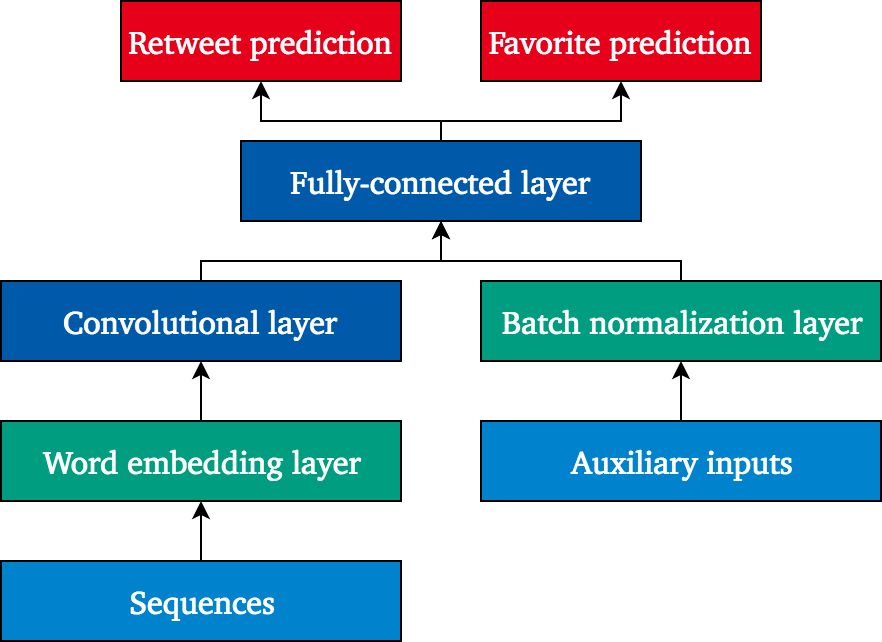
\includegraphics[width=.95\linewidth]{img/dm2_cnn}
  \caption{DM2-CNN}
  \label{fig:dm2_cnn}
\end{subfigure}%
\begin{subfigure}{.5\textwidth}
  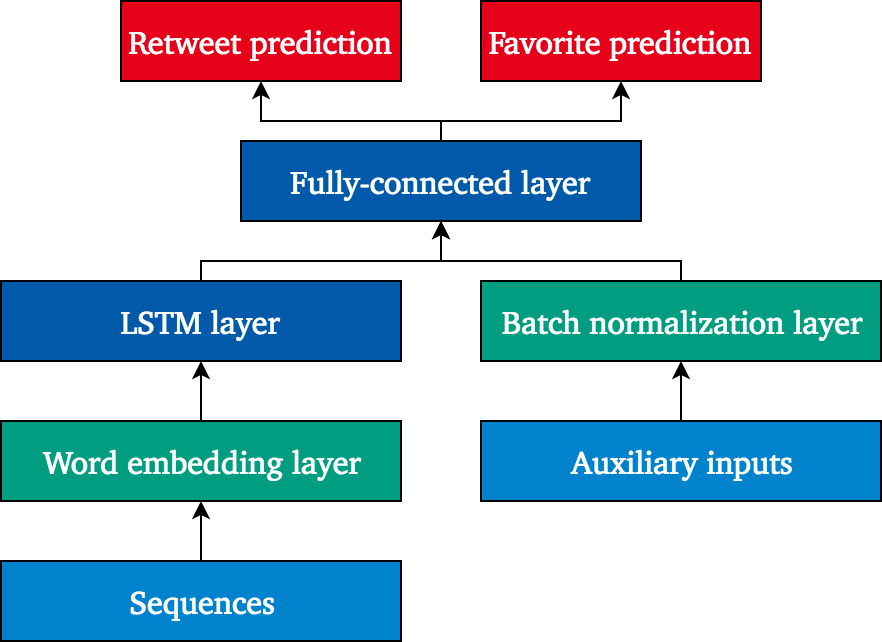
\includegraphics[width=.95\linewidth]{img/dm2_lstm}
  \caption{DM2-LSTM}
  \label{fig:dm2_lstm}
\end{subfigure}
\begin{subfigure}{.7\textwidth}
  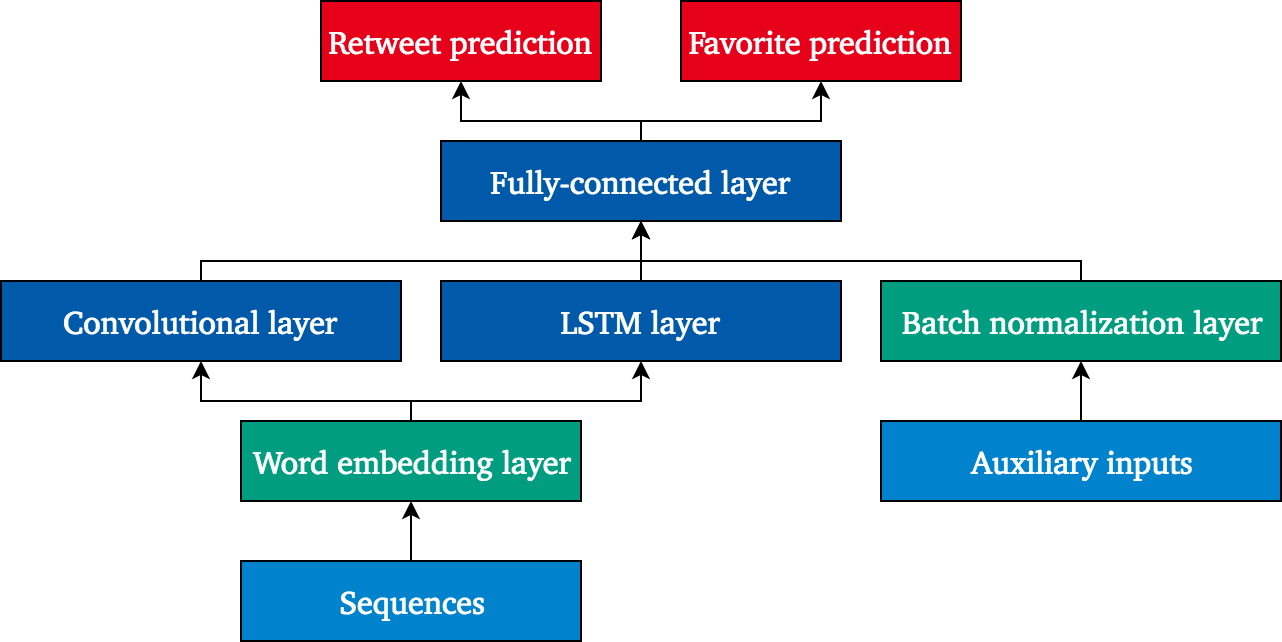
\includegraphics[width=.95\linewidth]{img/dm2_cnn_lstm}
  \caption{DM2-CNN-LSTM}
  \label{fig:dm2_cnn_lstm}
\end{subfigure}
\caption{Subset of evaluated architectures for multi-input models}
\label{fig:dm2_architectures}
\end{figure}

Figure~\ref{fig:dm2_architectures} shows a subset of the evaluated architectures for
multi-input neural networks.
For the sake of brevity, models are identified using a shortcode (see subfigure captions).
As illustrated, \textit{DM2-CNN} processes textual inputs via a single convolutional
layer.
More specifically, 32 filters aim to detect features from three successive words
(thus, filter size is 3).
Prior to consumption by the convolutional layer, inputs are padded with one leading
and trailing zero in order to keep the sequence lengths static.
Max-pooling (see \ref{sub:dl_developments}) is applied following the convolutional layer,
i.e., outputs of neighboring sequence subsets are combined by only keeping the
maximum value.
This effectively widens the scope of all filters and halves the input sequence
for successive layers.
Not included in this figure are models \textit{DM2-CNN2} and \textit{DM2-CNN3},
which employ two respectively three consecutive convolutional layers to the
textual inputs.
In theory, this allows learning of more complex features.
\textit{DM2-LSTM} replaces convolutional layers with a single LSTM cell.
As described above, singular words are fed to this cell one-by-one.
After processing this smallest possible input unit, a 16-dimensional learned
representation is returned.
Thus, LSTM cells in these models return sequences, similar to convolutional layers.
The final architecture, called \textit{DM2-CNN-LSTM}, combines the above
architectures by applying both convolutional and LSTM layers to the inputs
in parallel.
Consequently, more features can be combined with the following fully-connected
layer.
A commonality of all evaluated architectures is that inputs are firstly fed to
a word embedding layer, which is also trainable.
This means, that the pre-trained word vectors derived from GloVe are updated
during each training iteration.
Intuitively, this allows shaping of these vectors to the specific problem of
engagement prediction.
The above models were regularized as needed, mainly by adding dropout after
convolutional layers.
Moreover, batch normalization was inserted after the fully-conntected layer and
to normalize the additional inputs.
Auxiliary inputs represent the same structured features from previous models,
output classes are also unchanged.

\begin{table}
\begin{tabular}{llrr}
\toprule
Model architecture & Data set & Classification loss & Regression loss \\
\midrule
DM2-CNN & Combined & 0.7897 & \textbf{401.5174} \\
DM2-LSTM & Combined & 0.7628 & 411.2176 \\
DM2-CNN-LSTM & Combined & \textbf{0.7556} & 410.8704 \\
DM2-CNN2 & Combined & 0.7641 & 409.1842 \\
DM2-CNN3 & Combined & 0.8050 & 404.9901 \\
\bottomrule
\end{tabular}
\caption{Summary of multi-input model selection}
\label{tab:dm2_selection_results}
\end{table}

The model selection process was undertaken on the combined data set, since it
comprises the highest number of examples and is thus least prone to overfitting.
Table~\ref{tab:dm2_selection_results} lists results of applying all evaluated
architectures to engagement classification and regression.
Presented loss values were calculated on the held-out validation data.
It becomes obvious that all models show similar performance, i.e., differences
between loss values are not that big.
However, most suitable architectures for both tasks can be identified.
The DM2-CNN architecture was chosen for further evaluation on the other data
sets.
As a sidenote, the trained model contains no regularization other than batch
normalization.
Furthermore, the combining fully-connected layer contains 64 neurons.
A more complex architecture, namely DM2-CNN-LSTM, was selected for the multi-class
classification problem.
Here, regularization via dropout was needed for improved generalization capabilities.
The size of the fully-connected layer was doubled to 128 neurons in order to
account for the larger number of features derived from the tweet content.
